\documentclass[a4paper,12pt]{article}

% Основные пакеты
\usepackage[utf8]{inputenc}             % Поддержка кодировки UTF-8
\usepackage[T1, T2A]{fontenc}           % Поддержка кириллицы
\usepackage[english, russian]{babel}    % Поддержка русского и английского языков
\usepackage{graphicx}                   % Для вставки изображений
\usepackage{import}                     % Для продвинутого импорта (например, из Inkscape)
\usepackage{subcaption}                 % Для создания подписей к изображениям в сетке
\usepackage{float}                      % Для улучшенного размещения изображений
\usepackage{geometry}                   % Для управления отступами на странице
\usepackage{amsmath, amssymb, amsfonts} % Для математических формул и символов
\usepackage{booktabs}                   % Для красивых таблиц
\usepackage[dvipsnames]{xcolor}         % Для расширенной поддержки цветов
\usepackage[colorlinks]{hyperref}       % Для создания гиперссылок
\usepackage{indentfirst}                % Для красной строки в первом абзаце
\usepackage{listings}                   % Для оформления листингов кода
\usepackage{longtable}                  % Для длинных таблиц
\usepackage{makecell}                   % Для улучшенного форматирования ячеек таблиц
\usepackage{multirow}                   % Для объединения строк в таблицах
\usepackage{tabularray}                 % Для продвинутых таблиц
\usepackage{varwidth}                   % Для переменной ширины блоков
\usepackage{bm}                         % Для жирных математических символов
\usepackage{pifont}                     % Для специальных символов (например, галочек)
\usepackage{fontawesome}                % Для иконок
\usepackage{tcolorbox}
% Настройка отступов на странице
\geometry{left=2cm, right=2cm, bottom=2cm, top=2cm}

% Настройка гиперссылок
\hypersetup{
    linkcolor=blue,
    filecolor=magenta,
    urlcolor=cyan
}

% Настройка листингов
\definecolor{codegreen}{rgb}{0,0.6,0}
\definecolor{codegray}{rgb}{0.5,0.5,0.5}
\definecolor{codepurple}{rgb}{0.58,0,0.82}
\definecolor{backcolour}{rgb}{0.95,0.95,0.92}

% Определим стиль для выделения переменных
\lstdefinestyle{codestyle}{
	backgroundcolor=\color{backcolour},  % Цвет фона
	commentstyle=\color{codegreen}\itshape,  % Стиль для комментариев
	keywordstyle=\color{magenta}\bfseries,  % Стиль для ключевых слов
	numberstyle=\tiny\color{codegray},  % Стиль для номеров строк
	stringstyle=\color{codepurple},  % Стиль для строк
	identifierstyle=\color{black},  % Стиль для переменных (выделим их синим)
	basicstyle=\ttfamily\footnotesize,  % Размер шрифта для кода
	breakatwhitespace=false,  % Не разрывать строки в пробелах
	breaklines=true,  % Разбивать длинные строки
	captionpos=b,  % Позиция заголовка (внизу)
	keepspaces=true,  % Сохранять пробелы
	numbers=left,  % Позиция номеров строк
	numbersep=10pt,  % Расстояние между кодом и номерами строк
	showspaces=false,  % Не показывать пробелы
	showstringspaces=false,  % Не показывать пробелы в строках
	showtabs=false,  % Не показывать табуляции
	tabsize=4,  % Размер табуляции
	frame=single,  % Добавить рамку вокруг кода
	rulecolor=\color{black},  % Цвет рамки
	backgroundcolor=\color{backcolour},  % Цвет фона рамки
	xleftmargin=15pt,  % Отступ слева
	xrightmargin=15pt,  % Отступ справа
}

\lstset{style=codestyle, extendedchars=\true}

% Путь к изображениям
\graphicspath{ {./images/} }

\begin{document}
\begin{titlepage}
    \centering
    \vspace*{1cm}

    {\large Министерство науки и высшего образования Российской Федерации}\\
    {\large ФЕДЕРАЛЬНОЕ ГОСУДАРСТВЕННОЕ АВТОНОМНОЕ ОБРАЗОВАТЕЛЬНОЕ УЧРЕЖДЕНИЕ ВЫСШЕГО ОБРАЗОВАНИЯ «НАЦИОНАЛЬНЫЙ ИССЛЕДОВАТЕЛЬСКИЙ УНИВЕРСИТЕТ ИТМО»}\\
    {\large (УНИВЕРСИТЕТ ИТМО)}\\

    \vspace{2cm}

    {\large Факультет «Систем управления и робототехники»}\\

    \vspace{3cm}

    \textbf{{\Huge ОТЧЕТ}\\
    {\Huge О ЛАБОРАТОРНОЙ РАБОТЕ №4}}\\

    \vspace{1cm}

    {\LARGE По дисциплине «Техническое зрение»}\\
    {\LARGE на тему: «Сегментация изображений»}\\

    \vspace{2cm}

    {\Large Студент:}\\
    Охрименко Ева ИСУ 409290\\

    \vspace{2cm}

    {\Large Преподаватель:}\\
    Шаветов Сергей Васильевич\\

    \vspace{4cm}

    {\large г. Санкт-Петербург}\\
    {\large 2025}

\end{titlepage}

\tableofcontents  % Оглавление
\newpage

\section{Цель работы}

Освоение основных способов сегментации изображений на семантические области.


\section{Task. Бинаризация.}

\subsection{Бинаризация по двойному диапазону}

Итак, в этом задании нужно сделать бинаризацию, воспользовавшить формулой:
\begin{align*}
    I_{\text{new}}(x,y) = 
    \begin{cases} 
    0, & I(x,y) \leqslant t_1, \\
    1, & t_1 < I(x,y) \leqslant t_2, \\
    0, & I(x,y) > t_2 
    \end{cases}
\end{align*}
где \(I\) - исходное изображение,  \(I_{\text{new}}\) - бинаризованное.
За \(t_i\) берутся пороги бинаризации. Напишу функцию, которая делает бинаризацию
изображения:


\begin{lstlisting}[language=Python, caption=Бинаризация по двойному диапазону]
def binarizazia(image, t1, t2):
    imageGray = cv2.cvtColor(image, cv2.COLOR_BGR2GRAY)
    roi = np.uint8((imageGray >= t1) & (imageGray <= t2)) * 255
    return roi
\end{lstlisting}

Применим эту функцию к этой картинке:

\begin{figure}[H] % [H] - точное позиционирование
    \centering % Выравнивание по центру
    
\includegraphics[width=0.5\linewidth]{im/im.jpg} % Путь к файлу
    \caption{Исходный торт} % Подпись снизу
    \label{fig:my_image} % Метка для ссылок
\end{figure}

\begin{figure}[H]
    \centering
    \begin{subfigure}[b]{0.3\textwidth}
      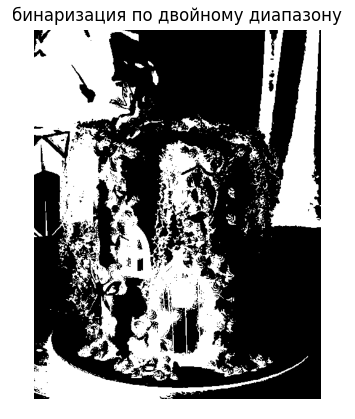
\includegraphics[width=\linewidth]{im/bin1.png}
      \caption{\(t_1 = 0, t_2 = 100\)}
    \end{subfigure}
    \hfill % Горизонтальный отступ
    \begin{subfigure}[b]{0.3\textwidth}
      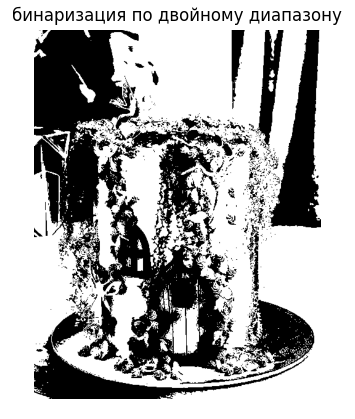
\includegraphics[width=\linewidth]{im/bin2.png}
      \caption{\(t_1 = 100, t_2 = 200\)}
    \end{subfigure}
    \hfill
    \begin{subfigure}[b]{0.3\textwidth}
      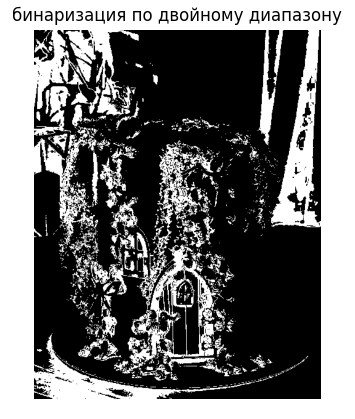
\includegraphics[width=\linewidth]{im/bin3.png}
      \caption{\(t_1 = 50, t_2 = 100\)}
    \end{subfigure}
    \caption{Бинаризация по двойному диапазону для разных \(t\)}
\end{figure}


Получается отчерно-белила картинку по разным пороговым значениям.


\subsection{Автоматическая бинаризация}

В этом задании нужно найти порог бинаризации как среднее арифметичческое
между максимальной интенсивностью и минимальной:
\[
t = \frac{I_{\text{max}} - I_{\text{min}}}{2}
\]
Вот код:
\begin{lstlisting}[language=Python, caption=Бинаризация \(t\) = среднее]
def binarizazia(image, t1, t2):
    imageGray = cv2.cvtColor(image, cv2.COLOR_BGR2GRAY)
    roi = np.uint8((imageGray >= t1) & (imageGray <= t2)) * 255
    return roi
\end{lstlisting}

В расчетах получилось \(t = 127.5\). Применяем к моей картинке такую бинаризацию:

\begin{figure}[H] % [H] - точное позиционирование
    \centering % Выравнивание по центру
    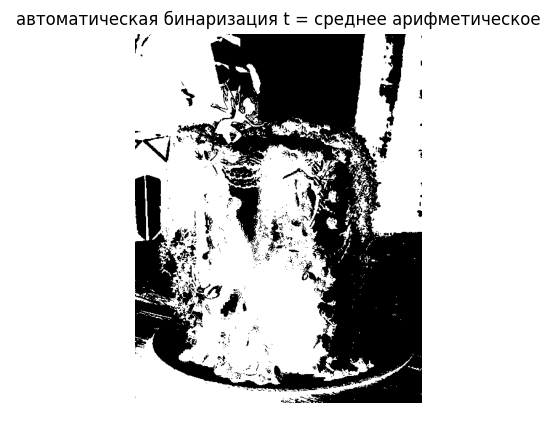
\includegraphics[width=0.8\linewidth]{im/bin4.png} % Путь к файлу
    \caption{} % Подпись снизу
    \label{fig:my_image} % Метка для ссылок
\end{figure}


\subsection{Бинаризация. Вычисление оптимального \(t\)}

Итак, в этом задании мне нужно найти оптимальное \(t\) по формулам
на основе модуля градиента яркости каждого пикселя. 
Для этого сначала вычисляем модуль градиента в каждой точке \( (x, y) \):

\[
G(x,y) = \max \left\{ \left| I(x+1, y) - I(x-1, y) \right|, \left| I(x, y+1) - I(x, y-1) \right| \right\}
\]

затем вычисляем оптимальный порог \( t \):

\[
t = \frac{\sum\limits_{x=0}^{X-1} \sum\limits_{y=0}^{Y-1} I(x,y) G(x,y)}{\sum\limits_{x=0}^{X-1} \sum\limits_{y=0}^{Y-1} G(x,y)}
\]


Вот такая функция у меня получилась:

\begin{lstlisting}[language=Python, caption=оптимальное \(t\)]
def binarizaziaOptimzeT(image):
    image = cv2.cvtColor(image, cv2.COLOR_BGR2GRAY)
    gradX = np.abs(image[2:, 1:-1] - image[:-2, 1:-1])
    gradY = np.abs(image[1:-1, 2:] - image[1:-1, :-2])
    G = np.zeros_like(image, dtype=np.float32)
    G[1:-1, 1:-1] = np.maximum(gradX, gradY)
    numerator = np.sum(image * G)
    denominator = np.sum(G)
    t = numerator / denominator if denominator != 0 else 0.0

    _, result = cv2.threshold(image, t, 255, cv2.THRESH_BINARY)
    return result
\end{lstlisting}

Оптимальное \(t\) получилось 118.39. Посмотрим на бинаризованный рисунок:
\begin{figure}[H] % [H] - точное позиционирование
    \centering % Выравнивание по центру
    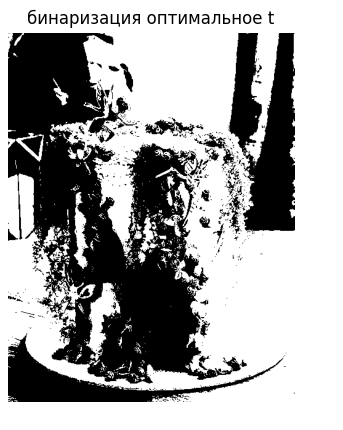
\includegraphics[width=0.5\linewidth]{im/bin5.png} % Путь к файлу
    \caption{} % Подпись снизу
    \label{fig:my_image} % Метка для ссылок
\end{figure}


\subsection{Бинаризация. Вычисление \(t\) методом Отсу}

И наконец вычислим \(t\) методом Отсу. Для этого 

\[
\omega_1(k) = \sum_{s=0}^{k} p_s, \quad \omega_2(k) = \sum_{s=k+1}^{L} p_s
\]
\[
\mu_1(k) = \frac{\sum_{s=0}^{k} s \cdot p_s}{\omega_1(k)}, \quad \mu_2(k) = \frac{\sum_{s=k+1}^{L} s \cdot p_s}{\omega_2(k)}
\]
\[
\sigma_b^2(k) = \omega_1(k) \omega_2(k) (\mu_1(k) - \mu_2(k))^2
\]
\[
t = \arg \max_k \sigma_b^2(k)
\]

Теперь напишем код, который все это делает:


\begin{lstlisting}[language=Python, caption=Метод Отсу]
def binarizaziaStatisticNetodOzy(image):
    image = cv2.cvtColor(image, cv2.COLOR_BGR2GRAY)
    hist = cv2.calcHist([image], [0], None, [256], [0, 256])
    hist = hist.flatten() 
    N = image.size 
    p_i = hist / N
    sigmaMax = t = 0
    for k in range(1, 256):
        w1 = np.sum(p_i[:k+1])
        w2 = 1 - w1
        if w1 < 1e-10 or w2 < 1e-10:
            continue
        mu1 = np.sum(np.arange(k+1) * p_i[:k+1]) / w1
        mu2 = np.sum(np.arange(k+1, 256) * p_i[k+1:]) / w2
        sigmaQuad = w1 * w2 * (mu1 - mu2)**2
        if sigmaQuad > sigmaMax:
            sigmaMax = sigmaQuad
            t = k
    _, result = cv2.threshold(image, t, 255, cv2.THRESH_BINARY)
    return result
\end{lstlisting}


Этим методом \(t\) получилось 117. Посмотрим на бинаризованный рисунок:

\begin{figure}[H] % [H] - точное позиционирование
    \centering % Выравнивание по центру
    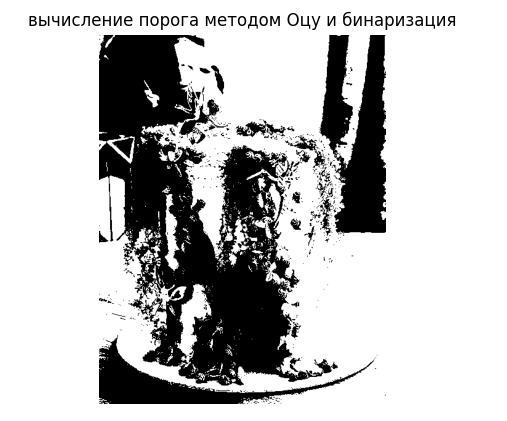
\includegraphics[width=0.6\linewidth]{im/bin6.png} % Путь к файлу
    \caption{} % Подпись снизу
    \label{fig:my_image} % Метка для ссылок
\end{figure}

\section{Task. Сегментация лица. (Не)питерская расчлененка}
В этом задании я воспользуюсь сегментацией изображений по принципу Вебера
\[
W(I) =
\begin{cases} 
\frac{20 - 12I}{88}, & 0 \leq I \leq 88, \\
0.002(I - 88)^2, & 88 < I \leq 138, \\
\frac{7(I - 138)}{117} + 13, & 138 < I \leq 255.
\end{cases}
\]

Алгоритм заключается в том, чтобы найти несколько похожих по интенсивности классов
пикселей и наделть похожие пиксели из одного класса одним цветом.

Было сложно, но я написала такие две функции:

\begin{lstlisting}[language=Python, caption=Сегментация по Веберу]
def weber(i):
    if 0 <= i <= 88:
        return 20 - (12 * i) / 88
    elif 88 < i <= 138:
        return 0.002 * (i - 88)**2
    elif 138 < i <= 255:
        return 7 * (i - 138) / 117 + 13
    else:
        return 0

def segment(image):
    image = cv2.cvtColor(image, cv2.COLOR_BGR2GRAY)
    segmented = image.copy()
    n = 0
    iN = 0
    while iN <= 255:
        w = weber(iN)
        upperBound = min(iN + w, 255)
        mask = (image >= iN) & (image <= upperBound)
        segmented[mask] = min(n * 30, 255)
        iN = upperBound + 1
        n += 1
        if upperBound == 255:
            break
    return segmented
\end{lstlisting}

Заценим исходное и получившееся изображения:


\begin{figure}[H]
    \centering
    \begin{subfigure}[b]{0.45\textwidth}
      
\includegraphics[width=\linewidth]{im/im2.jpg}
      \caption{Исходное изображение}
    \end{subfigure}
    \hfill % Горизонтальный отступ
    \begin{subfigure}[b]{0.45\textwidth}
      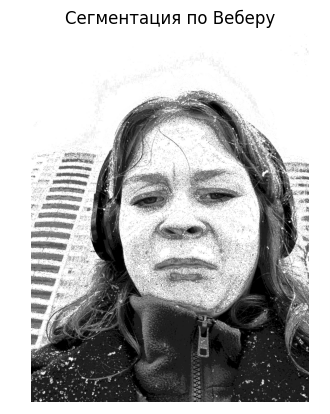
\includegraphics[width=\linewidth]{im/seg.png}
      \caption{Полученное изображение}
    \end{subfigure}
    \caption{Сегментация по Веберу}
\end{figure}

Можно наблюдать недовольного автора и недовольно-сегментированного. Сегментация прошла
успешно, даже лицо в крапинку получилось, хотя на исходной фотографии веснушки слабозаметны.




\section{Task. Сегментация методом \(k-means\)}

Метод \(k\)-средних — это алгоритм кластеризации, который делит данные на \(k\) кластеров. Алгоритм работает следующим образом:
\begin{enumerate}
    \item Сначала случайным образом выбираются \(k\)(хотя не совсем случайным, в моем коде
    это передаваемый в функцию параметр) центров кластеров.
    \item Каждый объект (пиксель изображения) присваивается ближайшему центру.
    \item Затем пересчитываются новые центры кластеров как среднее значение объектов в каждом кластере.
    \item Шаги 2 и 3 повторяются до тех пор, пока центры кластеров не перестанут изменяться.
\end{enumerate}

Напишу функцию для этого метода:
\begin{lstlisting}[language=Python, caption=Сегментация \(k-means\)]
def kMeans(image, k):
    image = cv2.cvtColor(image, cv2.COLOR_BGR2RGB)
    imageLab = cv2.cvtColor(image, cv2.COLOR_RGB2Lab)
    L, a, b = cv2.split(imageLab)
    ab = np.stack((a.flatten(), b.flatten()), axis=1)
    kmeans = KMeans(n_clusters=k, random_state=42, n_init=3)
    labels = kmeans.fit_predict(ab)
    labels_2D = labels.reshape(image.shape[:2]) 
    segmentedImages = []
    for i in range(k):
        mask = (labels_2D == i)
        segment = np.zeros_like(image)
        segment[mask] = image[mask]
        segmentedImages.append(segment)
    return segmentedImages
\end{lstlisting}

Посмотрим, что получилось для этой картинки:

\begin{figure}[H] % [H] - точное позиционирование
    \centering % Выравнивание по центру
    
\includegraphics[width=0.8\linewidth]{im/im3.jpg} % Путь к файлу
    \caption{Яблочки} % Подпись снизу
    \label{fig:my_image} % Метка для ссылок
\end{figure}

И для разных значений \(k\):


\begin{figure}[H]
    \centering
    \begin{subfigure}[b]{01\textwidth}
      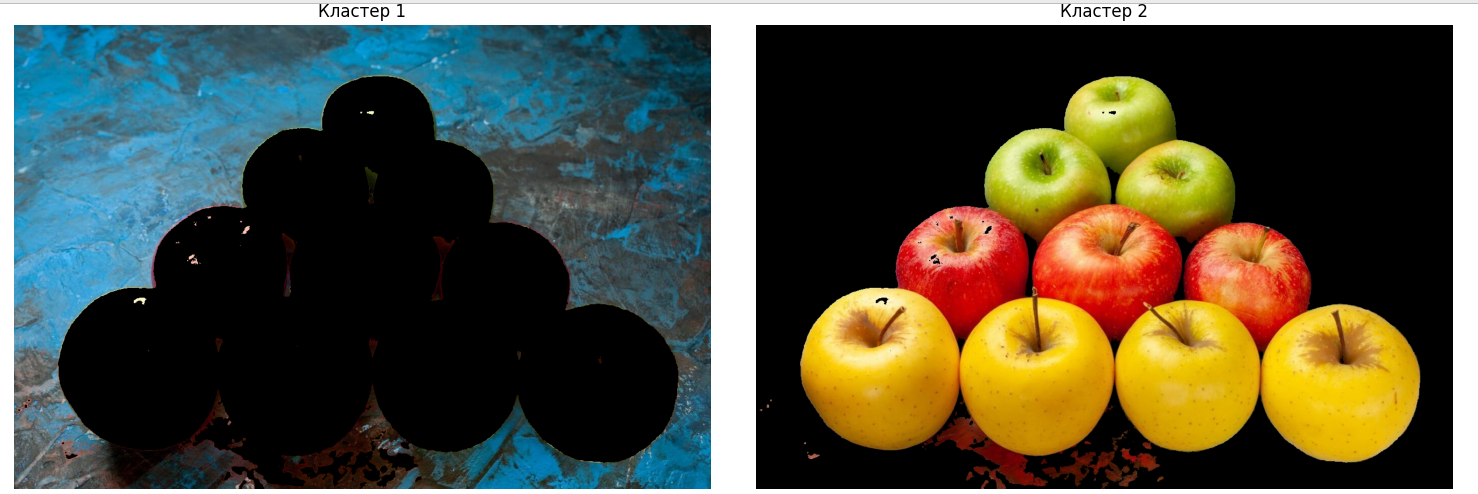
\includegraphics[width=\linewidth]{im/k2.png}
      \caption{\(k = 2\)}
    \end{subfigure}
    \hfill % Горизонтальный отступ
    \begin{subfigure}[b]{1\textwidth}
      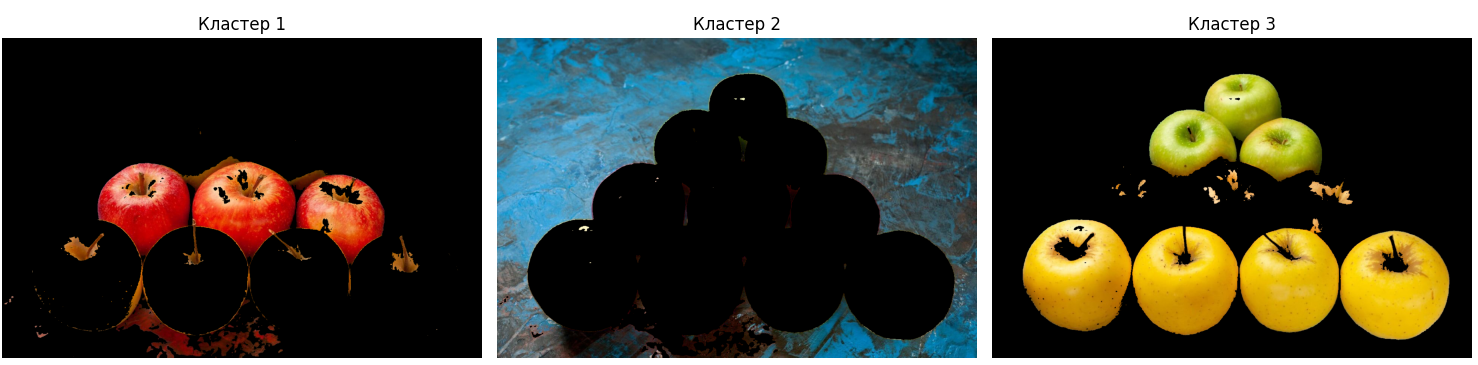
\includegraphics[width=\linewidth]{im/k3.png}
      \caption{\(k = 3\)}
    \end{subfigure}
    \hfill % Горизонтальный отступ
    \begin{subfigure}[b]{1\textwidth}
      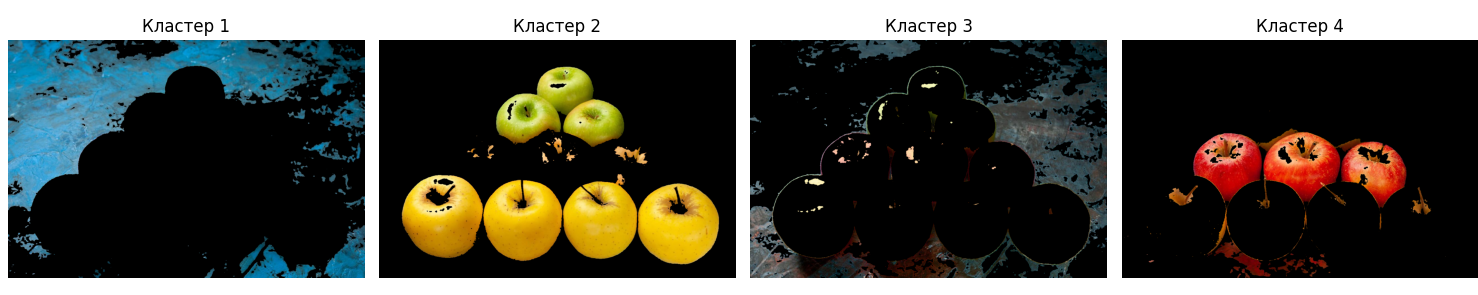
\includegraphics[width=\linewidth]{im/k4.png}
      \caption{\(k = 4\)}
    \end{subfigure}
    \caption{Сегментация методом \(k-means\)}
\end{figure}


Все успешно сегментируется на похожие цвета.


\section{Текстурная сегментация}

В этом задании нужно выбрать произвольное изображение, содержащее две разнородные текстуры. Выполнить текстурную сегментацию изображения, оценить не менее трех параметров выделенных текстур, определить к какому классу относятся текстуры.

Для этого я

\begin{itemize}
	
	\item Вычислю и нормализую энтропию для локальных областей размером $9 \times 9$ пикселей:
		
			$$E(x,y) = -\sum_{i=0}^{255} p_i \log_2 p_i$$
			где $p_i$ - вероятность интенсивности $i$ в окрестности точки $(x,y)$.
			$$E_{\text{norm}} = \frac{E - E_{\min}}{E_{\max} - E_{\min}}$$
	\item Сделаю бинаризацию  методом Оцу
	
	\item Для каждой связной компоненты $C_i$ проверю площадь $A_i$:
	
		$$
		BW(x,y) = 
		\begin{cases}
			0, & \text{если } (x,y) \in C_i \text{ и } A_i < 2000 \\
			BW(x,y), & \text{иначе}
		\end{cases}
		$$
		
		\item Морфологическое закрытие 
		$$\text{closed} = (BW \oplus K) \ominus K$$
		
		\item Построение маски по контурам 
		$$\text{mask}(x,y) = 
		\begin{cases}
			255, & \text{если } (x,y) \text{ внутри любого контура} \\
			0, & \text{иначе}
		\end{cases}$$
		
	\item Напишу код:
	
	\begin{lstlisting}[language=python, caption={Текстурная сегментация}]
def texture_segmentation(I):
	E = rank.entropy(I, rectangle(9, 9))
	E_norm = (E - E.min()) / (E.max() - E.min())
	_, BW = cv2.threshold(np.uint8(E_norm * 255), 0, 255, cv2.THRESH_BINARY + cv2.THRESH_OTSU)
	
	num_labels, labels, stats, _ = cv2.connectedComponentsWithStats(BW, 8, cv2.CV_32S)
	for i in range(1, num_labels):
		if stats[i, cv2.CC_STAT_AREA] < 2000:
			BW[labels == i] = 0
	
	kernel = np.ones((9,9), np.uint8)
	closed = cv2.morphologyEx(BW, cv2.MORPH_CLOSE, kernel)
	contours, _ = cv2.findContours(closed, cv2.RETR_CCOMP, cv2.CHAIN_APPROX_SIMPLE)
	mask = np.zeros_like(closed)
	cv2.drawContours(mask, contours, -1, 255, -1)
	
	return mask
\end{lstlisting}


	
\end{itemize}

Теперь я разделю  исходное изображения на две текстуры с помощью маски, полученной из функции 

	\begin{lstlisting}[language=python, caption=]
image = cv2.imread('../images/im4.jpg', cv2.IMREAD_GRAYSCALE)
mask = texture_segmentation(image)
texture1 = image.copy()
texture1[mask != 255] = 0
texture2 = image.copy()
texture2[mask == 255] = 0
\end{lstlisting}


Далее сделаю анализ текстур, красивый \texttt{plot} и вывод:

\begin{lstlisting}[language=python, caption={Вывод}]
def analyze_texture(img, name):
	glcm = graycomatrix(img, [1], [0], symmetric=True, normed=True)
	contrast = graycoprops(glcm, 'contrast')[0, 0]
	energy = graycoprops(glcm, 'energy')[0, 0]
	homogeneity = graycoprops(glcm, 'homogeneity')[0, 0]
	print(f"\n{name}:")
	print(f"Контраст: {contrast:.4f}")
	print(f"Энергия: {energy:.4f}")
	print(f"Однородность: {homogeneity:.4f}")
	
	return contrast, energy, homogeneity

params1 = analyze_texture(texture1, "Текстура 1")
params2 = analyze_texture(texture2, "Текстура 2")

plt.figure(figsize=(15, 5))
plt.subplot(131), plt.imshow(image, cmap='gray'), plt.title('Оригинал')
plt.subplot(132), plt.imshow(texture1, cmap='gray'), plt.title('Текстура 1')
plt.subplot(133), plt.imshow(texture2, cmap='gray'), plt.title('Текстура 2')
plt.tight_layout()
plt.show()

def classify_texture(contrast, energy, homogeneity):
	if contrast < 5 and energy > 0.8:
		return "Гладкая"
	elif contrast > 10 and energy < 0.5:
		return "Шершавая"
	else:
		return "Средняя"

print("\nКлассификация:")
print("Текстура 1:", classify_texture(*params1))
print("Текстура 2:", classify_texture(*params2))
\end{lstlisting}

Вот что у меня получилось:

\noindent
\fbox{
	\begin{minipage}{\dimexpr\linewidth-2\fboxsep-2\fboxrule\relax}
		\vspace{0.5em} 
		
		Текстура 1: \\
		Контраст: 307.5683 \\
		Энергия: 0.4779 \\
		Однородность: 0.5374 \\
		
		Текстура 2: \\
		Контраст: 94.1663 \\
		Энергия: 0.5204 \\
		Однородность: 0.7862 \\
		
		Классификация: \\
		Текстура 1: Шершавая \\
		Текстура 2: Средняя 
		
		\vspace{0.5em} 
	\end{minipage}
}
\\

\begin{figure}[H]
	\centering
	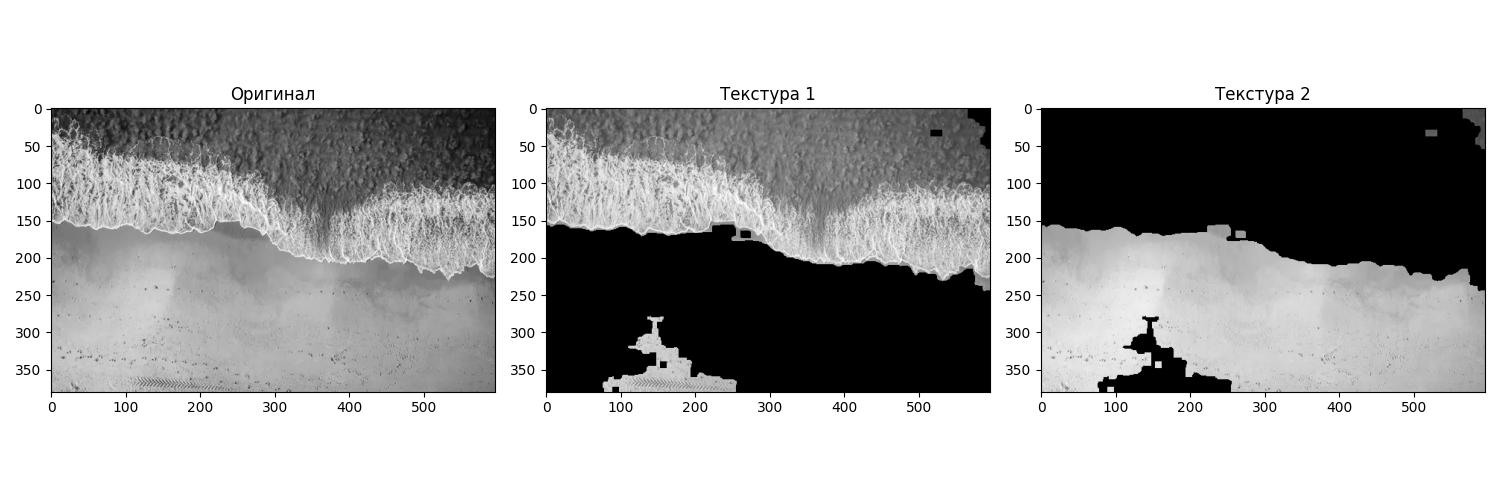
\includegraphics[width=1\linewidth]{im/im5.jpeg}
	\caption{Текстурная сегментация} % Подпись снизу
	\label{fig:my_image} % Метка для ссылок
\end{figure}


\section{Вопросы}


\begin{enumerate}
	\item В каких случаях целесообразно использовать сегментацию по принципу Вебера? 
	
	--- Сегментация по Веберу полезна, когда освещение неровное — например, если на фото есть тени или блики.
	
	\item Какие значения имеют цветовые координаты \textbf{a} и \textbf{b} цветового пространства \textbf{CIE Lab} в полутновом изображении?
	
	--- В полутоновом изображении $a = 0$ и $b = 0$, так как там нет цветовой информации, только яркость $L$.
	
	\item Зачем производить сегментацию в цветовом пространстве
	\textbf{CIE Lab}, а не в исходном \textbf{RGB}?
	
	--- Сегментация в \textbf{CIE Lab} лучше, чем в \textbf{RGB}, потому что она отделяет яркость \textit{L} от цвета \textit{a, b}, что делает её устойчивой к изменению освещения
	
	\item Что такое \textit{цветовое пространство} и \textit{цветовой охват}?
	
	--- Цветовое пространство — это система кодирования цветов (например, \textbf{RGB}), а цветовой охват — диапазон цветов, который оно или устройство может отобразить.
\end{enumerate}

\section{Вывод}

Эксперименты подтвердили, что для сегментации изображений важно подбирать методы под конкретную задачу. Автоматические алгоритмы (как Оцу или K-means) работают быстро и почти без настроек, что удобно для практики. Большинство задач удалось решить успешно, а результаты показали, что изученные методы действительно полезны.

Текстурная сегментация хорошо отделяет участки с разной структурой — например, воду от песка на снимках. Главный плюс: она учитывает не только цвет, но и узоры, что помогает там, где обычные методы не справляются. 	\href{https://github.com/decadeos/ITMO/tree/master/2_course/texViz/lab4}{GitHub}.
\end{document}